%%%%%%%%%%%%%%%%%%%%%%%%%%%%%%%%%%%%%%%%%%%%%%%%%%%%%%%%%%
%
% Vzor pro sazbu kvalifikační práce
%
% Západočeská univerzita v Plzni
% Fakulta aplikovaných věd
% Katedra informatiky a výpočetní techniky
%
% Petr Lobaz, lobaz@kiv.zcu.cz, 2016/03/14
%
%%%%%%%%%%%%%%%%%%%%%%%%%%%%%%%%%%%%%%%%%%%%%%%%%%%%%%%%%%

% Možné jazyky práce: czech, english
% Možné typy práce: BP (bakalářská), DP (diplomová)
\documentclass[czech,BP]{thesiskiv}

% Definujte údaje pro vstupní strany
%
% Jméno a příjmení; kvůli textu prohlášení určete, 
% zda jde o mužské, nebo ženské jméno.
\author{Hinterholzinger Jan}
\declarationmale

%alternativa: 
%\declarationfemale

% Název práce
\title{Softwarová podpora organizace předmětů TSP}

% 
% Texty abstraktů (anglicky, česky)
%
\abstracttexten{The text of the abstract (in English). It contains the English translation of the thesis title and a short description of the thesis.}

\abstracttextcz{Text abstraktu (česky). Obsahuje krátkou anotaci (cca 10 řádek) v češtině. Budete ji potřebovat i při vyplňování údajů o bakalářské práci ve STAGu. Český i anglický abstrakt by měly být na stejné stránce a měly by si obsahem co možná nejvíce odpovídat (samozřejmě není možný doslovný překlad!).
}

% Na titulní stranu a do textu prohlášení se automaticky vkládá 
% aktuální rok, resp. datum. Můžete je změnit:
%\titlepageyear{2016}
%\declarationdate{1. března 2016}

% Ve zvláštních případech je možné ovlivnit i ostatní texty:
%
%\university{Západočeská univerzita v Plzni}
%\faculty{Fakulta aplikovaných věd}
%\department{Katedra informatiky a výpočetní techniky}
%\subject{Bakalářská práce}
%\titlepagetown{Plzeň}
%\declarationtown{Plzni}

%%%%%%%%%%%%%%%%%%%%%%%%%%%%%%%%%%%%%%%%%%%%%%%%%%%%%%%%%%
%
% DODATEČNÉ BALÍČKY PRO SAZBU
% Jejich užívání či neužívání záleží na libovůli autora 
% práce
%
%%%%%%%%%%%%%%%%%%%%%%%%%%%%%%%%%%%%%%%%%%%%%%%%%%%%%%%%%%

% Zařadit literaturu do obsahu
\usepackage[nottoc,notlot,notlof]{tocbibind}

% Umožňuje vkládání obrázků
\usepackage[pdftex]{graphicx}

% Odkazy v PDF jsou aktivní; navíc se automaticky vkládá
% balíček 'url', který umožňuje např. dělení slov
% uvnitř URL
\usepackage[pdftex]{hyperref}
\hypersetup{colorlinks=true,
  unicode=true,
  linkcolor=black,
  citecolor=black,
  urlcolor=black,
  bookmarksopen=true}

% Při používání citačního stylu csplainnatkiv
% (odvozen z csplainnat, http://repo.or.cz/w/csplainnat.git)
% lze snadno modifikovat vzhled citací v textu
\usepackage[numbers,sort&compress]{natbib}

\usepackage{float}
\usepackage{dirtree}

% Barvičky
\usepackage{xcolor}
\colorlet{mygray}{black!30}
\colorlet{mygreen}{green!60!blue}
\colorlet{mymauve}{red!60!blue}
% Vkládání formátovaného zdrojového kódu
\usepackage{listings}
\renewcommand{\lstlistingname}{Ukázka kódu}
\renewcommand\lstlistlistingname{Seznam ukázek kódu}
\lstset{
	backgroundcolor=\color{gray!10},  
	basicstyle=\ttfamily,
	columns=fullflexible,
	breakatwhitespace=false,      
	breaklines=true,                
	captionpos=b,                    
	commentstyle=\color{mygreen}, 
	extendedchars=true,              
	frame=single,                   
	keepspaces=true,             
	keywordstyle=\color{blue},      
	language=php,                 
	numbers=none,                
	numbersep=5pt,
	numberbychapter=false,
	numberstyle=\tiny\color{blue}, 
	rulecolor=\color{mygray},        
	showspaces=false,               
	showtabs=false,
	showstringspaces=false,
	stepnumber=1,                  
	stringstyle=\color{mymauve},    
	tabsize=3,                      
	title=\lstname,
	numbers=left      
}

%%%%%%%%%%%%%%%%%%%%%%%%%%%%%%%%%%%%%%%%%%%%%%%%%%%%%%%%%%
%
% VLASTNÍ TEXT PRÁCE
%
%%%%%%%%%%%%%%%%%%%%%%%%%%%%%%%%%%%%%%%%%%%%%%%%%%%%%%%%%%
\begin{document}
%
\maketitle
\tableofcontents
\chapter{Úvod}
\section{Motivace}
	\par Na Katedře informatiky a výpočetní techniky vzniká nový předmět \uv{Týmový softwarový projekt} (KIV/TSP1 a KIV/TSP2) určený pro studenty navazujícího studia. Podstatou předmětu je vypracování zadaného tématu ve skupinkách studentů, kdy studenti přijdou do styku s týmovou prací, řízením projektu a dalšími interními procesy.
	\par Zvláštností předmětu je doba pro řešení projektu, dva semestry rozdělené do dvou předmětů. Budou zapojeny čtyři skupiny lidí. Garant, zadavatelé, mentoři a studenti, což bude klást poměrně značné nároky na organizaci předmětu. Pro takový rozsah bylo rozhodnuto o vytvoření webové aplikace, která všem zúčastněným stranám zjednoduší prohlížení obsahu a evidenci postupu prací projektu. Cílem aplikace je umožnit lepší informovanost a zapojení studentů, řešení evidence zadavatelů a možnosti sdílení mezi mentorem a garantem. Aplikace tak má nahradit způsob organizace pomocí Excel tabulky, jako je tak tomu u jiných obdobných předmětů.
\section{Cíl práce}
	\par Cílem práce je vyvinout zmíněnou webovou aplikaci dle specifikace předmětu a požadavků jeho garanta. Předpokládá se, že aplikace bude v budoucnu nadále rozšiřována. Je proto žádoucí, aby aplikace byla dostatečně robustní a důkladně otestována.
\chapter{Specifikace požadavků}
\par Specifikace požadavků se řídí průběhem a organizací předmětů TSP. V době vývoje aplikace se díky aktivní přípravě těchto předmětů několikrát požadavky změnily a tedy muselo být počítáno s průběžnou aktualizací specifikace. Díky tomu je potřeba aplikaci psát s dostatečným odstupem a přiměřeně obecně, aby odolávala drobným změnám specifikace.
\section{Organizace předmětů TSP}
	\par Výuka předmětů TSP je rozdělena do dvou semestrů, a tedy do dvou předmětů KIV/TSP1 vyučovaného v letním semestru 1. ročníku a KIV/TSP2 v zimním semestru 2. ročníku. Řešení týmového projektu tedy bude překračovat hranice ročníku a v mnoha částech se organizace předmětů bude překrývat.
	\par Jednotlivý cyklus se v nejčastějším případě bude probíhat následovně. 
	\begin{itemize}
		\item Garant přijímá od domluvených zadavatelů jejich témata, která mají studentské týmy řešit. Toto zadání společně s možným PDF souborem vloží do podpůrného softwaru pro zvolené období předmětu.
		\item Před začátkem TSP budoucí vedoucí týmu zažádá garanta o založení účtu v podpůrném softwaru s rolí \uv{Vedoucí}. Vedoucí týmu společně s dalšími studenty sestaví tým a vloží informace o týmu do této podpory.
		\item Poté co jsou témata zadání projektů zveřejněny, vedoucí týmu (na základě rozhodnutí v týmu) projeví zájem o zvolené téma.
		\item Mentor ohodnotí vhodnost zvoleného tématu pro daný tým na základě zájmu, který vedoucí týmu učinil.
		\item Garant následně podle rozhodnutí mentora a zájmu týmu definitivně přiřadí nebo nepřiřadí téma týmu. Přiřazením tématu vzniká projekt.
		\item Tým řeší projekt a postup řešení vkládá do softwarové podpory
		\item Mentor na základě postupu řešení týmu kontroluje a potvrzuje postup týmu
		\item Na závěru předmětu TSP se koná obhajoba projektu, jejíž výsledek se zapíše do softwarové podpory.
	\end{itemize}
\section{Uživatelé}
	\subsection{Nepřihlášený uživatel}
		\par Nepřihlášený uživatel je každý návštěvník aplikace, který se neprokáže svými přihlašovacími údaji. Takový uživatel může ve skutečnosti být student předmětu TSP, proto je mu umožněno zobrazovat vypsaná témata a týmy, které hledají nové členy.
	\subsection{Vedoucí týmu}
		\par Student předmětů TSP, který zažádal garanta o vytvoření konta. Tento uživatel je pověřen tvorbou týmu. Je mu umožněno vyjadřovat zájmy o volná zadání, které následně ohodnocuje mentor a na základě zájmu je garantem téma přiděleno. Také má možnost evidovat v projektu splnění kritérií, postupu a využitých zkušeností. Vedoucí vyplňuje údaje o týmu do softwarové podpory a eviduje postup projektu.
	\subsection{Mentor}
		\par Vyučující předmětů TSP, který má v softwarové podpoře založený účet- Jeho úkolem je evidovat postup a kontrolovat výstupy z týmu. Uživateli dále bude umožněno převzít si téma, které bude mentorovat a určovat vhodnost tématu dle vytvořených zájmů týmů o konkrétní téma, které mentoruje.
	\subsection{Garant}
		\par Garant je osoba, která koordinuje činnost všech ostatních skupin uživatelů. Mezi jeho hlavní náplní patří také přidávání nových témat, správa uživatelů a dalších nastavení softwarové podpory.

\chapter{Dostupné technologie}
\section{PHP}
\par PHP je jedním z nejoblíbenějších jazyků zpracovávaného na straně serveru v oblasti webového vývoje. Jedná se volně dostupný skriptovací jazyk, který je spravován a vyvíjen skupinou vývojářů s názvem The PHP Group.
\par Jazyk PHP se většinou používá na straně serveru (backend). Po jeho zpracování jsou výsledky typicky zobrazovány webovým serverem. Takový server musí mít nainstalovaný modul PHP. Poté lze vkládat kód jazyka do značkovaného kódu jazyka HTML. Soubory s PHP kódem mají koncovku .php. Jazyk je možné provozovat na velké škále operačních systémů na všech platformách.
\par Díky své jednoduchosti bývá PHP častá volba pro vývoj webových aplikací. Poskytuje dostatečné množství funkcí, aby programátor nepotřeboval přecházet na jiný jazyk a vystačil si čistě s jazykem PHP. Jazyk je konkurentem pro jazyky jako ASP.NET, Java a Node.js, které se také zabývají webovým vývojem.
\par Díky velké popularitě jazyka vznikla velká komunita vývojářů, kteří převážně zdarma nabízejí pomoc na různých fórech \cite{PHPOkamzite}.
\section{Srovnání PHP Frameworků}
	\par Existuje několik cest jak webovou aplikaci vyvíjet. V základu se jedná o dva směry. Vyvíjení aplikace z již vytvořených komponent a tvorba od úplného počátku. Oba směry mají své výhody a nevýhody. Pro rozsáhlé systémy se však posledních několik let rozmáhá použití frameworků.
	\subsection{PHP Framework}
	\par PHP framework je platforma pro tvorbu webových aplikací. Obsahuje knihovny pro často používané činnosti. Tvoří tak základ, na kterém mohou vývojáři stavět svůj produkt. Tento přístup je často vítaný, protože umožňuje urychlení a sjednocení vývoje.
	\par PHP framework pro vývojaře totiž řeší celou řadu problémů. Příkladem mohou být různé optimalizační nástroje, DI\footnote{Dependency Injection - technologie vkládání závislostí} kontejner nebo komunikace s databází. Vývojář se tak může zaměřit na vývoj samotné logiky aplikace a nezabývat se příliš repetetivními a nízkoúrovňovými záležitostmi.
	\par Součástí frameworků bývají šablonovací enginy. Ty vývojář často může nebo nemusí použít. Případně může zvolit jiný, který mu vyhovuje. Šablonovací enginy slouží pro prezentaci dat z backendové části aplikace a tvoří tak stránku, kterou vidí uživatel. Některé šablonovací systémy obsahují vlastní funkce například pro úpravu textu, podmíněné vykreslování nebo cykly. Struktury které známe z jiných programovacích jazyků. Zde však slouží pro zmíněnou prezentaci dat.
	\subsection{Vybrané frameworky ke srovnání}
	\par V dnešní době již existuje spousta spolehlivých frameworků, které mohou být použity. Stále však ujímají na nejvyšších příčkách frameworky Symfony a Laravel. Oba frameworky jsou mírně rozdílné a rozhodnutí, který nasadit spočívá v druhu použití.
	\subsubsection{Laravel}
	\par Framework Laravel je možné považovat jako za ten nejrozšířenější. Mezi jeho hlavní východy patří jeho jednoduchost používání a rychlost. Pro svůj přístup k jednoduchému použití je Laravel doporučován jako vhodný pro začátečníky ale i pro profesionály. Framework se hodí pro vytváření méně komplexních projektů.
	\par Laravel využívá šablonovací engine Blade, který je standardně dodáván společně se samotným frameworkem. Tento engine umožňuje oproti jiným rozšiřovat PHP kód, a tak provádět různé jednoduché operace pro přizpůsobení dat k samotnému front-endu.
	\subsubsection{Symfony}
	\par Tento framework se vyznačuje zakládáním si na striktním dodržování nejen PHP standardů a snaží se maximálně využívat různé návrhové vzory. Díky tomu jsou komponenty frameworku robustnější, což může znamenat větší časovou náročnost, ale také výraznou stabilitu frameworku, a proto je vhodný pro použití na komplexnějších projektech. Další předností mohou být rozsáhlé možnosti pro vývojáře, který si může prostředí přizpůsobit svým potřebám. To však vyžaduje hlubší znalosti jazyka PHP a struktury frameworku. Pro nováčky se tedy Symfony více náročný na naučení.
	\par Jako výchozí šablonovací engine je využíván Twig, který se také řadí mezi nejpoužívanější šablonovací systémy. Oproti systému Blade obsahuje navíc další bezpečnostní vrstvu a další funkce. Twig je často využíván i samostatně, tedy bez použití back-end frameworku. To podtrhuje jeho flexibilitu.
	\subsubsection{Nette}
	\par Český projekt Nette není tolik světově známý, ale v České republice je velice populární. Kombinuje totiž výhody obou předchozích frameworků a dosahuje velmi dobrých výsledků v rychlosti. Svoji popularitu si nadále udržuje i díky velmi aktivní komunitě.
	\subsection{Srovnání}
	\par Jedná se o frameworky, které každý
	\subsubsection{Podobnosti}
	\par Všechny zmíněné frameworky používají při komunikaci s databází objektově relační mapování. To znamená, že výsledky z databáze nejsou vráceny jako pole hodnot, ale jako objekty nad kterými lze volat další funkce. Díky tomu je možné dotazy na databázi i postupně optimalizovat a tím zrychlovat činnost aplikace.
	\par V otázkách poskytování závislostí všechny nabízejí vlastní formu DI kontejneru.
	\par Přikládané šablonovací enginy poskytují formu dědičnosti šablon. Umožňují rozšíření vlastními funkcemi a tak upravovat výpisy.
	
\section{PHP frameworky}
	\par Existuje mnoho úspěšných PHP frameworků, které mají různé typy zaměření. Mezi nejúspěšnější a nejpoužívanější patří Laravel, Symfony a Nette. Všechny tyto frameworky si zakládají na vytváření znovupoužitelných komponent a služeb. Kromě toho v sobě obsahují rozsáhlé nástroje pro usnadnění například práce s databází, přesměrování, ošetření bezpečnosti, atd. Díky tomu ulehčují vývojářům vlastní vývoj aplikace a nemusí tak vyvíjet úsilí pro tvorbu vlastních řešení. Výrazné zjednodušení představuje funkce dependency injection, která zajišťuje propojení mezi jednotlivými komponentami a službami a hlídá dostupnost všech závislostí.
	\par Součástí těchto frameworků jsou také šablonovací enginy, které zjednodušují tvorbu front-endu. Tyto šablonovací systémy umožňují dědičnost jednotlivých pohledů, jejich členění na sekce a obecně jejich cílem je jednodušeji prezentovat data z back-endu. Jednotlivé šablonovací enginy se liší svými funkcemi a rozšířeními, ale typicky je vybíráme dle osobních preferencí nebo dle použitého back-end frameworku.
\subsection{Nette}
	\par 
	\par S frameworkem společně přichází i šablonovací engine Latte.
\section{Front-end}
	\subsection{HTML a CSS}
		\par Základem webových aplikací je způsob zobrazování. Webové technologie nabízejí tvorbu elementů pomocí formátu HTML\footnote{Hyper Text Markup Language - Značkovací jazyk pro tvorbu webových technologí} založeného na XML\footnote{Extensible Markup Language - Víceúčelový značkovací jazyk}. Vlastností tohoto formátu je tvorba webových elementů pomocí tagů, kterým se specifikují jejich vlastnosti. Dnes již naprostá většina prohlížečů zobrazuje webové stránky pomocí tohoto formátu a stává prakticky synonymem pro internetové stránky \cite{HTML5aCSS3}.
		\par Další obdobně oblíbenou technologií je stylovací kaskádový jazyk CSS\footnote{Cascading Style Sheet - technologie pro úpravu vzhledu nejen webových stránek}. Díky tomuto formátu je možné nastavovat atributy jednotlivých elementů a upravovat tak zejména jejich vzhled. Tyto styly lze aplikovat přímo do HTML tagu daného elementu nebo do blokového elementu společný pro celou stránku. Nejčastěji se však využívá importování přiloženého \texttt{.css} souboru. CSS umožňuje vzhled stránky upravovat i podle velikosti displeje zařízení a tak přizpůsobit obsah i pro menší obrazovky \cite{CSSOkamzite}.
		\par Hlavním cílem jazyka CSS je oddělovat formátovací a stylizační pravidla od obsahu stránky. Díky tomu je možné stránky snadněji udržovat a přinutit je pracovat správně v různých webových prohlížečích, na různých platfomách, zařízení nebo dokonce při tisku \cite{HTML5aCSS3}.
	\subsection{Bootstrap}
		\par Bootstrap představuje nadstavbu nad CSS styly. Umožňuje upravovat prvky pomocí tříd a dát jim tak moderní vzhled bez potřeby upravovat styly ručně. Při správném použití tohoto frameworku je velice snadno zajištěn responzivní design webu.
	\subsection{AdminLTE}
		Ačkoli Bootstrap přichází již s hotovou sadou stylů pro určité prvky a pro responzivitu, tak stavba celé webové aplikace by se neobešla bez četného přidávání vlastních stylů. Existují však nástavby nad technologií Boostrap a nabízejí kompletní sadu stylů k vytvoření informačních systémů. Jedním z takových projektů je front-endový framework AdminLTE. 
		\par Tento framework nabízí celou řadu placených šablon, ale poskytuje i jednu velmi oblíbenou šablonu zdarma. Součástí tohoto frameworku jsou příklady použití stylů jednotlivých elementů a také předpřipravené šablony pro celé stránky.
		\par Framework využívá Bootstrap, je tedy stejně jednoduché využívat responzivitu a čerpat jeho dalších výhod. Stylování stránek tedy vypadá tak, že na hotovou HTML strukturu aplikujeme třídy, na které se následně navazují styly těchto frameworků. 
\section{Databáze MariaDB}
	\par Databáze je důležitá součást informačního systému, která zpracovává nějaká data a je potřeba jejich uložení a rychlé přístupnosti k nim.
	\par MariaDB databáze je relační databáze oblíbená vývojáři zejména webových projektů malé a střední velikosti. Systém MariaDB původně vznikl jako alternativní větev MySQL od původních vývojářů po zakoupení firmy Sun společností Oracle. MariaDB staví na své značné kompatibilitě s databází MySQL, která je považována z různých průzkumů za jednu z nejoblíbenějších databází pro webové aplikace společně s databází Oracle a MS SQL. Další přednosti systému MariaDB je její cíl zůstat open-source projektem.
	\par Díky velké kompatibilitě s databází MySQL je možné využívat nástroje určené nativně pro MySQL i pro MariaDB. Proto pro vývoj využíváme nástroj MySQL Workbench, který pro většinu případů poskytuje stejné funkce jako pro databázi MySQL.
\section{Nástroje pro řízení projektu}
	\par Aplikace, kterou vyvíjíme, bude patřit mezi rozsahově náročnější, proto je její řešení rozděleno do dvou prací. Jedna práce (tato) se věnuje samotnému vývoji aplikace. Druhá je zaměřená na důkladné otestování aplikace, čímž má být zajištěna její kvalita spolehlivost.
	\par Ze skutečnosti, že na aplikaci takového rozsahu pracuje více lidí, je potřeba využít takové procesy, které usnadní jednotlivé části vývoje a domluvu mezi vývojem, testováním a vedoucím práce.
\subsection{Verzovací systém}
	\par V oblasti vývoje informačních projektů je častým nástrojem pro efektivní a produktivní vývoj verzovací systém ze skupiny Git.
	\par Tato technologie totiž umožňují práci více vývojářů na jednom projektu současně. Jednotlivé změny v repozitáři vývojáři seskupují do tzv. commitů. Ty totiž v systémech Git představují nejmenší jednotku změny v úložišti. Commit v sobě obsahuje informace o upravených řádkách textových a změny dalších souborů.
	\par Další důležitou funkcí je větvení. V základu je v repozitáři hlavní větev \uv{main} nebo \uv{master}, který obsahuje centrální vývoj projektu. Od této větve se se oddělují další větve, dle určení. Typicky se do jednotlivých větví postupně commitují úpravy rozsáhlejší funkcionality aplikace. Díky tomu ostatní vývojáři nejsou těmito změnami zasaženi a tak si nepřekážejí.
	\par Po dokončení úprav nebo přidávání funkcionality jsou commity větve sloučeny do rodičovské větve, kde tvoří větší celek. Tato funkce se jmenuje Merge request a její starostí je přemístit commity jedné větve do jiné větve tak, aby byly změny zaneseny. Může se stát, že se změny v obou větvích dostanou do konfliktu, poté záleží na uživateli jak konflikt vyřeší.
	\par Dostupných nadstaveb verzovacích systémů existuje celá řada. Mezi nejvýznamnější na trhu patří GitHub a GitLab.
	\par GitHub je pravděpodobně nejúspěšnější systém pro tvorbu projektů od jednotlivců nebo malých skupin. Obsahuje však výrazná omezení, která jsou sice odstraněny v prémiovém plánu, ale v našem případě výhody ostatních nadstaveb převažují nad výhodami GitHubu.
	\par Z tohoto důvodu se zdá být přínosnější použít systém GitLab, který pokrývá veškeré naše požadavky. 
	\par Důležitou zmínkou je, že projekt GitLab je veden jako open-source. Díky tomu Katedra informatiky a výpočetní techniky provozuje svoji vlastní instalaci tohoto verzovacího nástroje na katedrálním serveru.
	\par To má pro studenty nesmírnou výhodu, protože během dosavadního studia již GitLab používali a mají s ním zkušenosti. Navíc všichni zúčastnění mají na této platformě vytvořené své účty, nemusíme tedy organizačně řešit vstup na novou platformu.
	\par Z těchto důvodů jsme se v naší volbě verzovacího systému rozhodli zvolit právě variantu s katedrálním serverem.
\subsection{Plánování úkolů}
	\par S rozsahem práce přichází i potřeba rozvržení práce na časové úseky a stanovení cílů. Zároveň je žádoucí, aby k plánu měli přístup všechny zúčastněné osoby. Tyto požadavky sice splňuje množství známých nástrojů nebo sdílených úložišť. My jsme se ale rozhodli využít již námi používaný nástroj GitLab.
	\par Tento nástroj obsahuje možnosti vytváření wiki dokumentace ve formátu MarkDown\footnote{Značkovací jazyk pro vytváření formátovaného textu}, který navíc zajišťuje základní formátování.
	\par V této dokumentátorské sekci máme vytvořenou jednu stránku, ve které je po týdnech rozdělena struktura naplánovaných úkolů a vzniklých dotazů.
\subsection{Issues}
	\par Různé požadavky evidujeme jako jednotlivé issues. Issues je záznam o požadavku na aplikaci nebo úkolu, který je potřeba vykonat. Issue tak eviduje přiřazení k člověku, který daný požadavek řeší, kompletní historii řešení požadavku, termíny pro jeho splnění, atd.
	\par Systém také poskytuje štítkování těchto issues a tím pomáhá v jejich řazení, filtrování, seskupování i výběru. Díky štítkům můžeme totiž přiřazovat prioritu, závažnost, druh požadavku na aplikaci a jiné označení.
	\par Issues nám pomáhají ve fragmentaci  jednotlivých požadavků na aplikaci do přibližně stejně náročných dílů, které se poté ve vývoji dobře plní a je tak zajištěna přehlednost. Zároveň má tento princip i pozitivní psychologický dopad, kdy vývojáři mají dobrý pocit z dokončeného úkolu a mají tak chuť pokračovat dalším issue.
	\par V systému GitLab tyto issues používáme také ve funkci Board, který využívá principy kanbanu.
\subsection{Kanban}
	\par Systém kanban je strategie řízení projektu, kdy si mezi sebou části výroby předávají výrobek. Cílem je využívat pouze ty nejnutnější zdroje.
	\par V praxi se tento systém zobrazuje jako tabule, kde jsou rozvržené jednotlivé sloupce dle možných stavů vývoje. Následně zde máme rámečky představující výrobek, které obsahují popis jak má být produkt upraven. Podstatou věci je, že tyto rámečky následně přemisťujeme mezi jednotlivými sloupci v závislosti na reálném stavu produktu.
	\par Obrázek \ref{fig:kanban} obsahuje snímek z reálného použití při vývoji. Jednotlivé issues jsou rozděleny do sloupců dle jejich stavu rozpracovanosti.
	\begin{figure}[H]
		\centering
		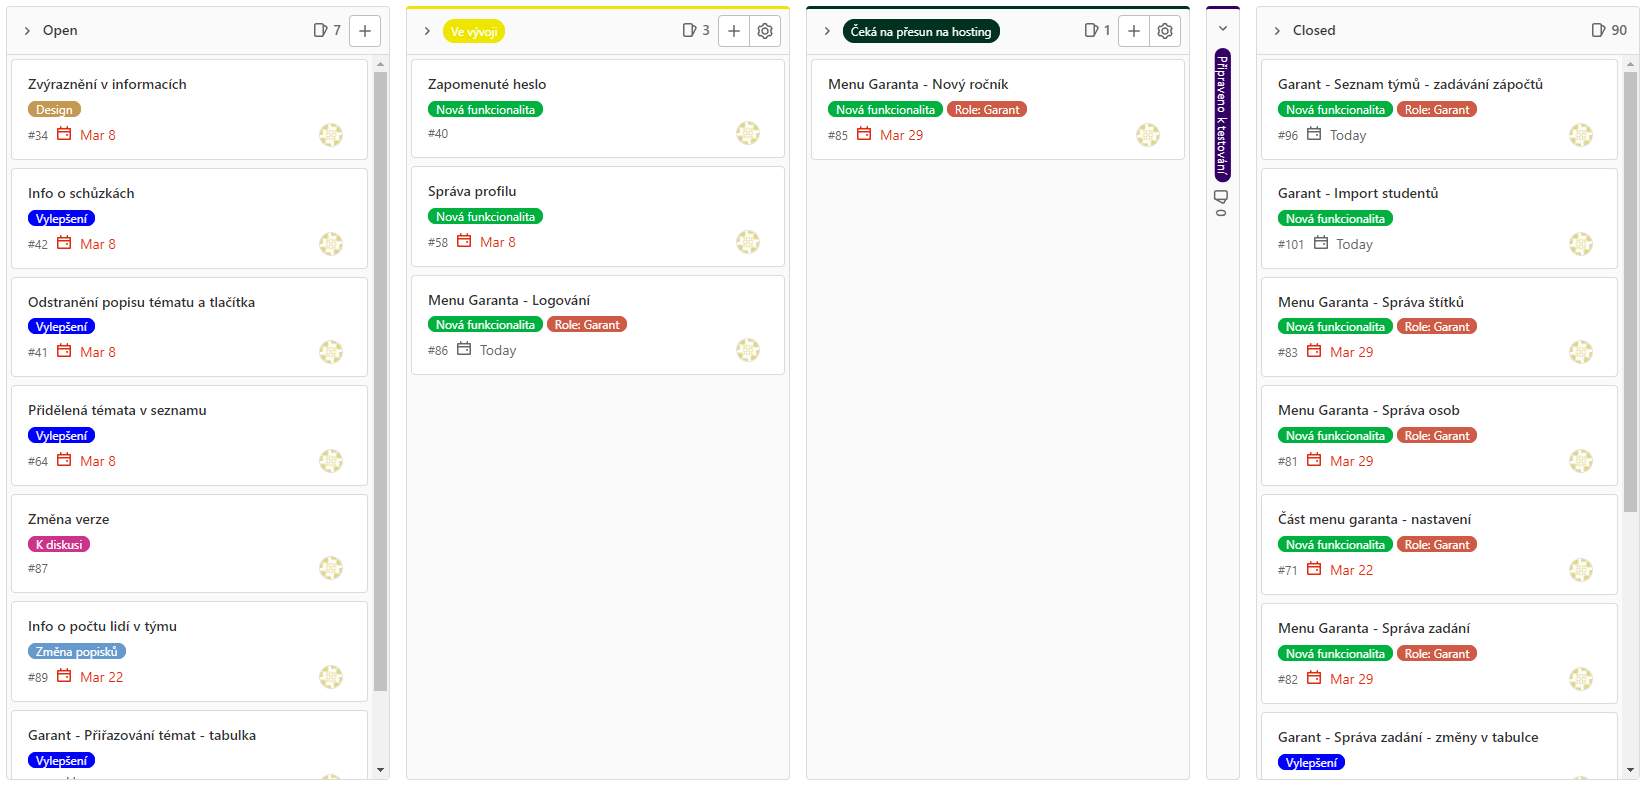
\includegraphics[width=\textwidth]{img/rizeni_projektu/kanban}
		\caption{Ukázka použití tabule s issues (zdroj: vlastní)}
		\label{fig:kanban}
	\end{figure}
	\par V informačních technologiích se kanban používá ve velké míře pro organizaci různých úkolů a požadavků. Různé části vývoje si mezi sebou požadavek vyměňují a tím mění jeho stav.
	\par Například když vývojář dokončí práci na nové funkcionalitě, tak přesune příslušný rámeček ze sloupce \uv{Ve vývoji} do sloupce \uv{Připraveno k testování}. Tím se tester dozví, že je daný úkol připraven k testování a může si úkol přiřadit a pracovat na něm.
	\par V GitLabu je systém kanbanu implementován v souvislosti s issues a jejich štítky. Každý issue je zobrazen jeden rámeček na tabuli kanban, kam se automaticky po vytvoření issue promítne a po přidělení štítků zařadí do připravených sloupců.
	\par Propojenost s issue nám ulehčí práci s přepisováním jednotlivých požadavků do jiných nástrojů, které mají obdobné funkce.
\subsection{MantisBT}
	\par Mantis Bug Tracker je webová aplikace pro nahlašování a evidenci chyb (defektů) vytvořených v průběhu vývoje aplikace. Přidávané defekty lze velmi podrobně popsat, určit prioritu a štítkovat.
	\par MantisBT využíváme pro nahlašování objevených selhání nalezených především, ale ne výhradně pomocí komplexního automatizovaného testování aplikace. Na základě reportování defektů jsou následně žádány jejich opravy chyb a po opravě jsou znovu testovány. Pro naše potřeby používáme vlastní instalaci MantisBT, která je přístupná pro anonymně přihlášené, aby mohli v budoucnu nahlašovat defekty i uživatelé aplikace.
\chapter{Návrh aplikace}

	\section{Dekompozice specifikace}
		\subsection{Zadání}
		\par V moment zveřejnění zadání pro mentory je mentorům umožněno zvolit si téma k mentorování. Po zvolení se automaticky přidělí danému mentorovi.
		\par Po úplném zveřejnění tématu je zadání zobrazováno ve veřejném seznamu témat. Vedoucí týmů mohou o takové zadání projevit zájem hodnotou na pětibodové stupnici vážnosti.
		\par Zadání se skládá z částí:
		\begin{itemize}
			\item název zadání
			\item stručný popis zadání
			\item PDF soubor s podrobným zadáním
			\item doporučovaná velikost týmu
			\item časová náročnost řešení
			\item kontaktní informace zadavatele
			\item požadovaný profil týmu.
		\end{itemize}
		\par Požadovaný profil týmu obsahuje štítky ze stejného souboru štítků jako v profilu týmu.
		\subsection{Tým}
		\par Tým je seskupení několika studentů. Má svého vedoucího, který vede tým a hájí jeho zájmy. Cílem týmu je řešení společného projektu na základě přiřazené tématu.
		\par Tým je vytvořem na požádání vedoucího garantem předmětu. Po vytvoření nového týmu se založí nový uživatelský účet pro vedoucího. Následně jsou vedoucímu na jeho studentský email zaslány přihlašovací údaje.
		\par Nastavení týmu provádí z zejména vedoucího týmu včetně přidávání studentů do týmu ze seznamu volných studentů zapsaných na předmět.
		\par Vedoucí týmu je zodpovědný za obsah, který do softwarové podpory vkládá.
		\subsection{Projekt}
	\section{Případy užití}
		\par Příklady užití popisují v krocích způsob používání různých částí aplikace uživatelem nebo systémem. Tyto případy představují se zadavatelem dohodnutou funkčnost systému. Vytvořené případy užití usnadňují tvorbu požadavků na systém pro následné sepsání testovacího plánu.
		\par Z podrobné specifikace požadavků byly sestaveny případy užití, které popisují práci s výslednou aplikací. Rozdělení případů užití jsou ilustrovány v use-case diagramu (viz obrázek \ref{fig:use-case}). Následuje seznam sestavených případů užití s popisem funkcí, které pokrývají.
		\subsection{Nepřihlášený uživatel}
			\subsubsection{Přihlášení (UC.01)}
				\par Velká část aplikace jsou přístupné pouze uživatelům dle jejich role. To vytváří potřebu autentizace v naší aplikaci. Uživatel má možnost se přihlásit pomocí přihlašovací stránky pomocí registrované kombinace přihlašovacího jména a hesla. Pokud je uživatel autentizován, je přesměrován na domovskou obrazovku pro jeho konkrétní roli.
			\subsubsection{Zobrazení témat (UC.02-03)}
				\par Nepřihlášený uživatel (např. běžný student) si může zobrazit seznam volných témat v přehledu, kde se dozví základní informace o tématech.
				\par Tyto témata lze rozkliknout do podrobnější podoby, kde je zobrazen název, stručný popis, časová náročnost, doporučená velikost týmu, zadavatel a mentor zadání. Také lze stáhnout PDF soubor s podrobným zadáním.
			\subsubsection{Neúplné týmy (UC.04)}
				\par Nepřihlášený uživatel má k dispozici seznam neúplných týmů, které hledají nové členy. Případný student má k dispozici seznam obsazených rolí a kontakt na vedoucího týmu.
		\subsection{Přihlášený uživatel}
			\subsubsection{Odhlášení (UC.05)}
				\par Přihlášený uživatel má možnost ukončit svou relaci a odhlásit se. Po této akci je uživatel přesměrován na hlavní stránku nepřihlášeného uživatele.
		\subsection{Vedoucí týmu}
			\subsubsection{Schůzky týmu (UC.06-09)}
				\par Vedoucí týmu může v aplikaci naplánovat schůzku. Schůzka může být obsahuje čas a místo konání a v jakém uskupení. Schůzka může být například interní, kdy tým se schází s jeho členy, aby například probrali další postup nebo může být za účasti mentora, zadavatele apod. Pokud je zvoleno, že se schůzky účastní mentor projektu týmu, zobrazí se schůzka kromě stránky týmu i na stránce mentorovaných projektů mentora.
			\subsubsection{Řešení projektu (UC.10-13)}
				\par V řešení projektu vedoucí týmu zaznamenává postup svého týmu pomocí čtyřstavové hodnoty v několika kategoriích. Na základě těchto záznamů přiřazený mentor kontroluje a potvrzuje tento postup týmu volbou ze stejného čtyřstavového výběru.
				\par Vedoucí týmu má na stránce řešení projektu možnost vyplnit a přidat užitečné odkazy.
			\subsubsection{Editace týmu (UC.14-16)}
				\par Vedoucí má možnost přidávat nebo odebírat členy týmu a signalizovat jednotlivé stavy týmu. Členům týmu může přiřazovat a odebírat týmové role. Také může vyplňovat týmový profil z předem definovaného seznamu schopností. Řádně stanovený profil dle opravdových schopností členů týmu může orientačně pomoci s výběrem tématu.
			\subsubsection{Stránka tématu a zájem o téma (UC.17-19)}
				\par Vedoucí jehož tým nemá přiřazené žádné téma může na stránce detailu volného zadání projevit zájem. Vážnost zájmu o téma je vybírána ze stupnice pěti hodnot od méně významné po nejvážnější. Vedoucí nemůže projevit zájem o téma s vážností, s kterou již má aktivní zájem o jiné téma.
				\par Projevené zájmy o témata (i ty neaktivní) jsou zobrazeny na stránce týmu, kde aktivní zájmy může vedoucí odvolat.
		\subsection{Mentor}
			\subsubsection{Změna kontaktních údajů (UC.20)}
				\par Mentor má ve správě profilu zpřístupněnou úpravu kontaktních údajů. Tyto údaje se následně zobrazují například u detailu zadání, kde je zobrazena \uv{vizitka} přiřazeného mentora.
			\subsubsection{Mentorované projekty (UC.21-25)}
				\par Jednou z hlavních tabulek mentora jsou mentorované projekty. V této tabulce uvidí o každém mentorovaném projektu stav řešení projektu v kompaktním zobrazení, datum přiřazení tématu týmu a samozřejmě prokliky na projekt a tým.
				\par Předpokládá se, že tato tabulka bude hlavním rozcestníkem mentora v průběhu mentorování projektů a tedy stránka na které se nachází je nastavena jako mentorova domovská stránka.
			\subsubsection{Schůzky (UC.09-10,26)}
				\par Mentor má přístup k vytváření schůzek týmů stejně jako vedoucí týmu. Navíc však disponuje tabulkou obsahující schůzky všech týmů, kterých má být mentor zúčastněný.
			\subsubsection{Volba tématu (UC.27-28)}
				\par Součástí navigace mentora je i položka \uv{Položka bez mentora} vedoucí na stránku s tabulkou témat, která nemají mentora. Tyto témata jsou buď zveřejněná pouze pro mentory nebo zcela veřejná. Témata z této nabídky si mohou mentoři v detailu zadání přiřadit k mentorování. Po přidělení je téma z tabulky odstraněno a naopak se objeví v tabulce \uv{Témata bez týmu}, pokud téma dosud není přiřazeno žádnému týmu, nebo na stránce \uv{Témata bez týmu}.
			\subsubsection{Témata bez týmu (UC.29-30)}
				\par Stránka témat bez týmu je rozdělena na dvě tabulky. Jedna tabulka obsahuje prostý výčet témat, která má mentor přidělené k mentorování, ale dosud žádný tým o ně neprojevil zájem. Druhá komplexnější tabulka obsahuje veškeré projevené zájmy týmu o zadání. Účel tabulky pochází ze specifikace, že mentor posuzuje vhodnost tématu pro daný tým. Výsledek posouzení mentor v příslušnému zájmu přidělí označení \uv{Nevhodné} nebo \uv{Vhodné}. Výchozí hodnota, kdy mentor dosud není rozhodnut je \uv{Neohodnoceno}.
			\subsubsection{Historie mentorování (UC.31)}
				\par Aplikace má v sobě udržovat historii předchozích ročníků TSP. Proto mentor má k dispozici výpis témat, která dosud mentoroval. Mentor se může na dané projekty prokliknout a prohlížet je.
		\subsection{Garant}
			\subsubsection{Témata bez mentorů}
			\par Garant vidí tabulku se seznamem témat, která nemají dosud přiřazeného mentora. Součástí tabulky je i název zadavatele.
			\subsubsection{Seznam týmů}
			\par Obdobná tabulka jako u pohledu mentora \uv{Mentorovaná tabulka}, obsahuje tedy podobné . Tabulka však navíc obsahuje i týmy, které nemají přiřazené žádné zadání. V tom případě tak proklik odkazuje na stránku týmu.
			\par Tabulka umožňuje přistoupit k editaci daného týmu, kde lze upravit údaje o týmu, zadávat datumy zápočtů a vytvářet záznamy o obhajobách.
			\subsubsection{Seznam mentorů}
			\par Stránka ukazující propojení témat a jejich mentorů mentorů. Proklikem na jméno mentora je mentor zvolen a garant může skrz navigační menu přistupovat k pohledům mentora.
			\subsubsection{Správa osob}
			\par Garant má k dispozici tabulky se seznamy všech uživatelů, kteří se mohou přihlásit. Tito uživatelé jsou rozděleni dle jejich role na mentory a vedoucí. Garant má oprávnění těmto uživatelům odebrat přístup čímž jim zamezí v jejich dalším přihlášení.
			\subsubsection{Správa témat}
			\par Garant má přístupnou tabulku všech zadání, kde o nich může vidět základní informace. 
			\par Součástí správy témat je i vytváření a editace nového zadání. Garant kromě všech dat zadání může přiřadit zadání mentora, určit ročník ve kterém je zadání vyvěšeno a upravovat jeho viditelnost.
			\subsubsection{Správa štítků}
			\par Používané štítky může garant také upravovat, vytvářet a znemožnit další použití. V aplikace jsou dva druhy štítků. Týmové role, které vedoucí přiřazuje členům jeho týmu a štítky pro profil týmu a zadání. Pokud garant pro jakýkoliv štítek nastavení, že není dostupný pro další užití, není možné jej nově použít. Naopak při znepřístupnění štítku není odebráno již stávající přiřazení, aby nebyla nijak upravována historie již proběhlých projektů.
			\subsubsection{Přidělování témat}
			\par Speciální tabulka, kde každý sloupec reprezentuje tým bez přiřazeného tématu a každý řádek jedno volné zadání. V tabulce jsou vyplněné ty buňky, kde existuje zájem týmu o dané zadání. Garant zde vidí vážnost zájmu a datum vytvoření zájmu. Zobrazuje se zde i doporučení mentora, které mentor vyplní na stránce \uv{Témata bez týmu}. Na základě těchto informací garant definitivně přiřadí zadání jednomu z přihlášených týmů.
			\subsubsection{Správa studentů}
			\par Na stránce správy studentů má garant k dispozici tabulku všech přidaných studentů. Z těchto studentů vedoucí vkládají členy do svých týmů. Garant může nad těmito studenty vyvolávat akce mazání a stanovení vedoucího nového týmu. Při vytvoření nového týmu je potřeba vyplnit počáteční název týmu. Studenti se do této tabulky přidávají buď jednotlivě pomocí formuláře nebo z přiloženého CSV\footnote{Comma-separated values - jednoduchý souborový formát pro výměnu tabulkových dat} souboru.
			\par Vkládání studenta jednotlivě vyžaduje znalost přihlašovacího jména do systému StaG, křestní jméno, příjmení, email, osobní číslo, ročník ve kterém je TSP studováno a případně obor studia se studovanou fakultou.
			\par Import studentů pomocí CSV umožňuje přidání velkého množství studentů najednou. Jedná se o vhodnou variantu pro hromadné přidávání studentů například na začátku semestru. Je počítáno s CSV souborem formátu, který poskytuje systém StaG při exportu studentů zapsaných na daný předmět. I v tomto případě je potřeba určit do kterého ročníku TSP importovaní studenti náleží.
			\subsubsection{Správa ročníků}
			\par Garant ve správě ročníků může vidět informace o jednotlivých proběhlých ročnících. Zároveň může tvořit nové ročníky a nastavovat aktuální ročník TSP. Po zvolení nového aktuální cyklu TSP se původní cyklus považuje za historický a je tak i zobrazován ve zbytku aplikace. Tímto způsobem je řešeno zachování předchozích ročníků TSP, kdy v běžném stavu aplikace se zobrazují zejména údaje vztažené k aktuálnímu ročníku TSP.
			\subsubsection{Logování}
			\par Pro sledování správní činnosti aplikace má garant přístup k zobrazení logovacích záznamů. Tato funkce je zprostředkována pomocí parsování sekvencí záznamů do tabulky. Garant si může zvolit logovací soubor k nabídky k jednoduchému zobrazení. Zvolený záznam může také stáhnout v textové podobě do počítače, kde s ním může provádět další operace.
		\begin{figure}[h]
			\centering
			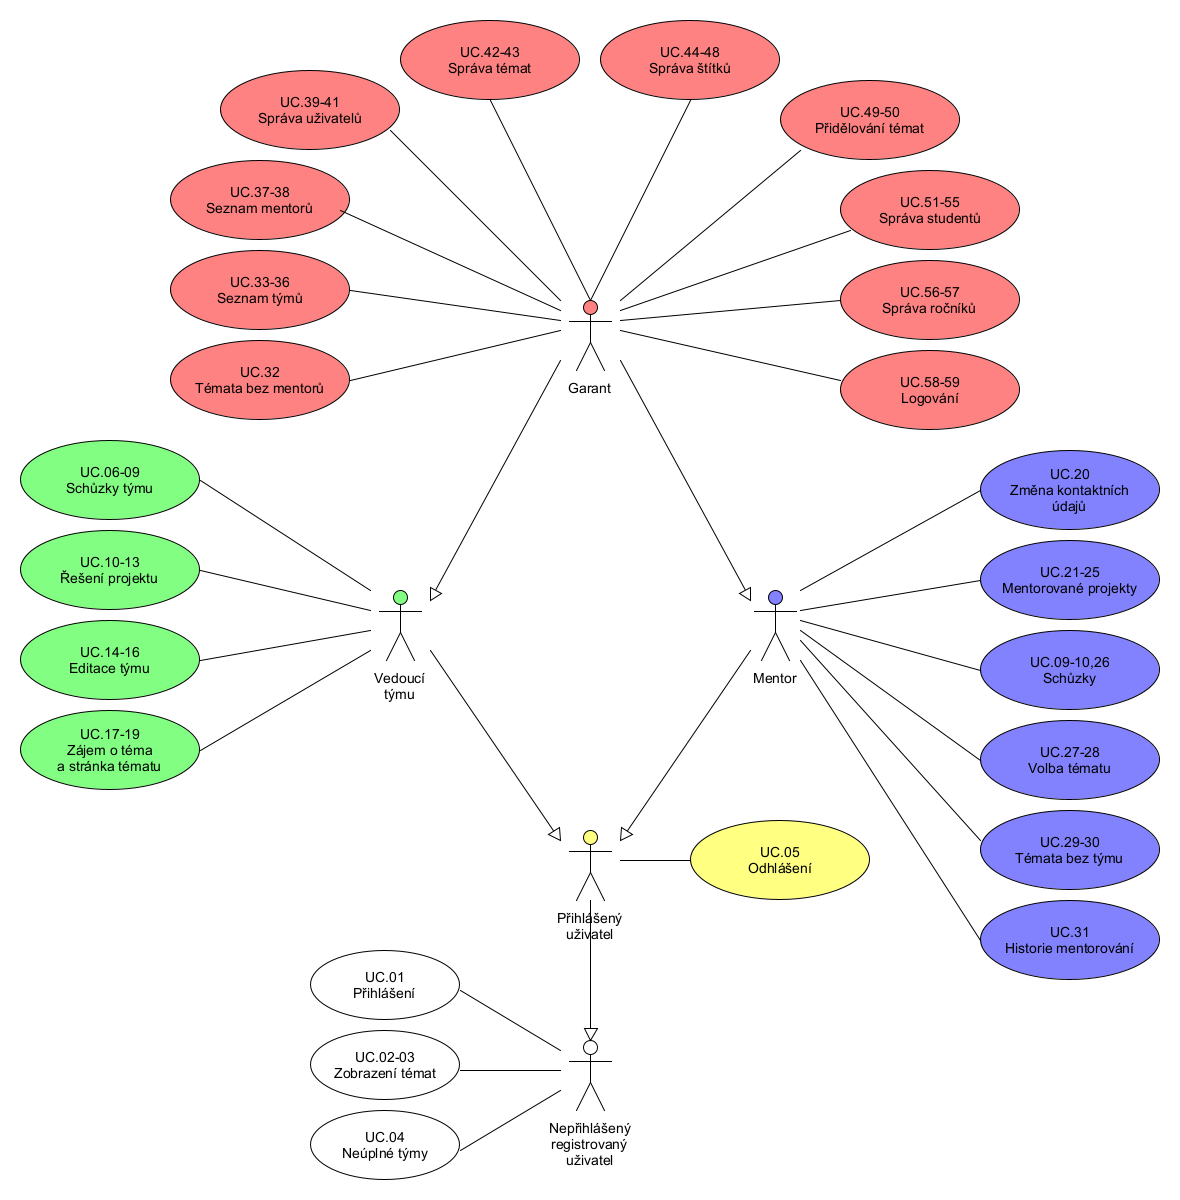
\includegraphics[width=0.8\textwidth]{img/use_case/use_case_diagram}
			\caption{Schéma případů užití (zdroj: vlastní)}
			\label{fig:use-case}
		\end{figure}
	\section{Architektura aplikace}
		\subsection{Třívrstvá architektura}
		
		\cite{3Vrstvy}
		\par Architektura MVP\footnote{Model-View-Presenter - třívrstvá architektura} je třívrstvový návrh struktury aplikace pro rozdělení souborů dle funkčnosti s ohledem na rozšiřitelnost. MVP architektura se skládá z datové části (model), která se stará o práci s daty a umožňují vytvářet abstrakci nad jednotlivými strukturami. Například jednotlivé akce s databází v kontextu dat se kterými aplikace pracuje. Další část je aplikační vrstva (presenter), která řídí chod aplikace, předává data z šablon do modelů a naopak. Poslední vrstvou je vrstva prezentační. Ta se skládá z jednotlivých šablon a prezentace dat. Představuje tak rozhraní, přes které uživatel komunikuje s aplikací.
		\par Mezi další velice rozšířenou architekturou patří MVC architektura. Hlavním rozdílem mezi MVP a MVC architekturami je, zpracovávání vstupů od uživatele. V MVP architektuře jsou vstupy obsluhovány prezentovací vrstvou.
		\subsection{Komponenty aplikace v Nette}
		\par Komponenty jsou části aplikace, které vkládáme do stránek. Nejčastěji se jedná o formuláře, tabulky a další objekty, které je možné používat opakovaně.
		\par Nette má v sobě vestavěný komponentový systém, který umožňuje komponenty vkládat na stránky a někdy dokonce do jiných komponent, kdy se tak tvoří tzv. komponentový strom. Velkou výhodou je, že se komponenta tvoří až tehdy, kdy je opravdu použita. To těží výhodu zejména zpracování AJAX požadavků, kde je typicky výsledkem operace pouze část stránky, kdy není komponenta využita. Díky tomu se vůbec nevytváří tím šetří výkon serveru.
		\par Komponenty se vytváření v továrních funkcích v presenteru. Tyto funkce mají prototyp \texttt{createComponent<Name>(): Control} \cite{NetteComponents}.
		
		\subsubsection{Ukázka tovární metody v presenteru}
		\begin{lstlisting}[caption={Ukázka tovární metody v presenteru}]
class DefaultPresenter extends Nette\Application\UI\Presenter
{
	protected function createComponentPoll(): PollControl
	{
		$poll = new PollControl;
		$poll->items = $this->item;
		return $poll;
	}
}
\end{lstlisting}
		
		\par Komponentu lze definovat přímo v tovární metodě, ale pro účely znovupoužitelnosti je možné pro komponentu vytvořit vlastní třídu dědící třídu \texttt{Nette\textbackslash Application\textbackslash UI\textbackslash Control}.
		
		\subsection{Dependency Injection v Nette}
		\par Vkládání závislostí je technika programování vedoucí k čistému a přehlednému kódu. Princip tohoto způsobu programování spočívá v předávání zdrojů, které konkrétní funkce nebo třída vyžaduje, aby splnila svoji úlohu. Cílem je zamezit získávání zdrojů přímo v daném objektu, kdy programátor bez žádné další informace neví jaký zdroj se získá a jak se získá. V těchto případech říkáme, že se vytváří v aplikaci skryté vazby, díky kterým vzniká nepřehledný a špatně udržitelný kód \cite{PHP-DI}.
		\par Pro implementaci DI se využívá tzv. Dependecy Container. Tento nástroj slouží k uchování instancí jednotlivých služeb a jejich vytváření, pokud se jedná o závislosti aktuálně potřebných částí aplikace.
		\par Nette pro implementaci Depencency Containeru využívá vlastní knihovnu Nette DI Container. Knihovna se stará o automatické generování a aktualizaci tříd kontejneru na základě konfiguračního souboru formátu NEON. Díky této technologii programátor nemá potřebu implementace vlastního řešení a může se soustředit na vývoj logiky aplikace. Při vytváření jednotlivých služeb však nesmí zapomenout tuto službu zaregistrovat zapsáním do konfiguračního souboru.
		\par Další technologií, kterou Nette využívá, je nástroj Autowire. Ten se stará o automatické předávání závislostí z dependency kontejneru do konstruktorů a parametrů dalších funkcí \cite{NetteDI}.
		
		\subsection{Formuláře v Nette}
		\par Formuláře jsou důležitou součástí webového systému. Jedná se o jednu z mála možností jak získat uživatelský vstup. Zároveň tak představují bezpečností riziko, které je nutno ošetřit. Typů útoků skrz uživatelský vstup přes formuláře je velké množství a jejich ošetření klade nemalé časové a znalostní na programátora. Také i proto je tvorba a validace formulářů je velmi rutinní činnost. Framework Nette proto přichází se svým řešením Nette Forms. Jedná se o možnost tvorby formulářů, kdy programátor definuje základní prvky formuláře a framework sám z těchto informací sestaví formulář. Výhodou tohoto přístupu spočívá v bezpečnosti. Nette Forms totiž validuje vstupy uživatele podle definovaných validačních pravidel a to jak na straně backendu, tak v případě připojených příslušných JavaScript skriptů i na straně frontendu. Aplikaci tedy komponenta vrátí validovaná data, která může bez starostí použít.
		\par Tvorba formuláře probíhá jako obyčejná komponenta. Tovární funkce vrací instanci třídy \texttt{Nette$\backslash$Application$\backslash$UI$\backslash$Form}. Funkce instanci vytvoří a postupně do ní přidává formulářové prvky, kterým lze definovat další různá pravidla nebo vlastnosti. Je také potřeba implementovat kód, který se spustí po nějaké události ve formuláři. Zejména je myšlena událost úspěšně odeslaného formuláře, kdy je pravděpodobně nutné vykonat nějakou akci aplikace (např. uložit data).
		\par Vytvořenou komponentu formuláře je možno automaticky vykreslit dle předem vytvořené šablony pomocí šablonovacího systému Latte a tak jednoduše vložit formulář do příslušné stránky. Je však ponechána možnost vytvoření si jednotlivých formulářových prvků v šabloně a dle identifikátoru je propojit s prvky v komponentě \cite{NetteDI}.
		
		\subsection{Database Explorer}
		\par
		
		\subsection{Testovatelnost aplikace}
		\subsubsection{Testování robot frameworkem}
		\par Aby bylo možné aplikaci automaticky otestovat je potřeba umožnit testovacímu softwaru ovládat aplikaci. Proto musí být veškeré ovládací prvky jednoznačně identifikovatelné. Toho docílíme zavedením jednoznačných identifikátorů vložených do atributu \texttt{id} daných elementů.
		\par Robor framework díky tomu je schopen nalézt požadovaný prvek stránky. Takto jednoznačně identifikovatelné není potřeba mít pouze akční prvky typu odkazu nebo tlačítka, ale také i dalších prvků stránky. Ty Robot framework potřebuje nalézt, aby z nich mohl číst data.
		\par Navržené automatické testování se na tuto vlastnost spoléhá např. při orientaci v aplikaci. Každá stránka s obsahem má svůj nadpis. Tento nadpis má jednoznačný identifikátor v celé aplikaci. Na základě této značky se při testování zjišťuje, zda je otevřena žádaná stránka. Obdobným způsobem dokáže také získat data z jednotlivých elementů, ke kterým se dostane, a může provést jejich kontrolu.
		
		\subsubsection{Jednotkové testování}
		\par Princip jednotkového testování je ověření nejelementárnějších procedur aplikace. V tomhle ohledu se práce vyvíjené webové aplikace se skládá z většinové části pouze z interpretace dat z a do databáze voláním funkcí Nette frameworku a tedy se nedostáváme na elementární úroveň, kterou můžeme jednotkově testovat. Avšak při vývoji byly vytvořeny pomocné procedury, které pomáhají se zpracováním dat (např. parsování). Tyto funkce jsou oddělené od logiky aplikace a jsou závislé pouze na svých vstupech. Pro těchto pár funkcí byly vytvořeny jednotkové testy, které ověřují jejich výstupy.
		
		\subsubsection{Logování}
		\par Logování je určené pro dlouhodobé sledování činnosti programu. V sekvenci záznamů je možné dohledat souvislosti zpracovaných akcí a stavu systému. Pomocí logování sledujeme zejména běžnou činnost programu, výskyt chyb a výjimek, konfiguraci programu a její změny. Tato technika lze být použita i pro ladění, ale v našem případě máme jiné ladící nástroje \cite{OKSPrednasky}.
		\par Pro PHP existuje profesionálně používaná knihovna Monolog\footnote{https://github.com/Seldaek/monolog}. Ta již integrována do známých frameworků jako Symfony, Laravel i Nette. Logovací záznam je pole o jednotlivých položkách např. úroveň, časové razítko, jméno loggeru, zaznamenávaná zpráva, dodatečn informace, atd. Tyto údaje však negeneruje programátor přímo, ale zpravidla pomocí logovacích funkcí loggeru.
		\par Záznamy loggerů ukládáme do adresáře \texttt{/log/syslog/} v textovém formátu \texttt{.log}. Záznamy jsou rozděleny do jednotlivých souborů dle dne a soubory s logy starší 30 dní jsou automaticky mazány. Veškeré tyto parametry lze změnit v konfiguraci aplikace a upravit tak logování dle zjištěných reálných potřeb systému.
		\subsubsection{Ladící nástroj Tracy}
		
		\subsection{Responzivita}
		\par Responzivní desing spočívá v přizpůsobení zobrazení obsahu šířce okna webového prohlížeče (příp. velikosti obrazovky zařízení). To znamená, že uživatel navštěvující naší stránku ze stolního počítače nebo mobilního zařízení uvidí uspořádaný obsah tak, aby byl na daném zařízení dostatečně čitelný a ovladatelný \cite{CSSOkamzite}.
		\par Front-end aplikace je implementován frameworkem AdminLTE, který staví na základech technologie Bootstrap. Díky tomu je snadné udržovat aplikaci responzivní pokud je dodržena správná HTML struktura a jsou důsledně aplikovány styly použitím tříd stylů.
		
		\subsection{Vícejazyčnost}
		\par Mezi požadavky na aplikaci je podpora vícejazyčného prostředí. Zejména byla vyžádána možnost přepnout rozhraní do anglického jazyka.
		\par Pro splnění tohoto požadavku byl implementován balíček \texttt{kdyby/translation}. Balíček umožňuje vkládat do šablon a kódu řetězce dle jejich identifikátoru ze souborů s překlady. Vždy se tak použije řetězec ze souboru dle aktuálně nastaveného jazyka.
		\par Soubory s překlady jsou uloženy ve formátu NEON ve vlastním adresáři. Každé jazykové podání je obsaženo v samostatném souboru. Hodnoty jednotlivých překladů jsou uspořádány v hierarchické struktuře. Pro vizuální i logické oddělení tak lze větvit strukturu dle částí aplikace, ve kterých jsou překlady řetězce obsaženy.
	
	\section{Databázová struktura}
		\par Struktura databáze musí obsahovat veškeré informace použitelné v softwarové podpoře a umožnit jejich snadné propojení. Dalších aspektem pro tvorbu struktury je použitý PHP framework, který využívá službu pro správu databázových dotazů a jejich optimalizaci. Pro jeho správnou funkci je potřeba mít strukturu databáze řádně připravenou včetně vytvořených indexů a propojení pomocí cizích klíčů.
		\par Databázová struktura musí respektovat, že požadavkem na aplikaci je prohlížení historie. To nás přivádí na strategii, že každá tabulka u které to bude potřeba bude provázána s tabulkou \texttt{PERIOD} jejíž řádky představují jednotlivé cykly TSP. Také se však vyskytuje problém u odstraňování záznamů. Prakticky nebude možné z databáze cokoli odstraňovat, aby nebyl porušen konzistentní stav již proběhlých projektů. To je následně ve struktuře zapracováno v různých tabulkách sloupcem s příznakem, který určuje zda je prvek odstraněn nebo znepřístupněn pro další užití. Tím prvek stále existuje, není porušeno integritní omezení a potřebné změny pro nové projekty jsou upraveny.
		
		\begin{figure}[H]
			\centering
			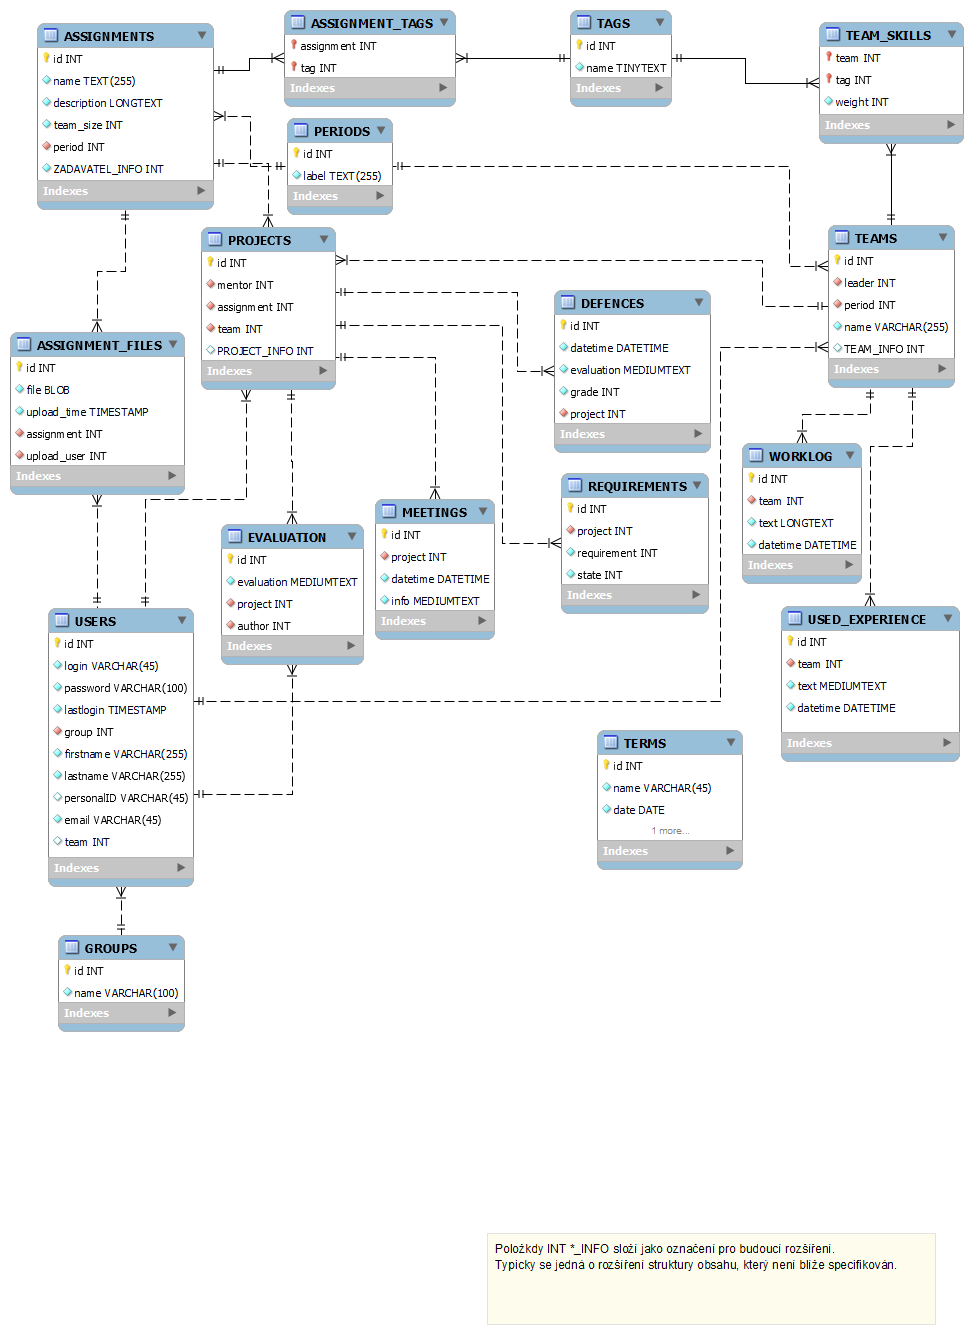
\includegraphics[width=0.8\textwidth]{img/database/database_model}
			\caption{Schéma databázové struktury (zdroj: vlastní)}
			\label{fig:strukturaDB}
		\end{figure}
		\subsection{Základní tabulky}
			\begin{itemize}
				\item USER -- Tabulka pro ukládání uživatelů, kteří mají/měli přístup do aplikace. Součástí této tabulky jsou přihlašovací údaje, role uživatele a následné propojení na další informace dle role uživatele.
				\item STUDENT -- Uživatelé s rolí \uv{Vedoucí} vycházejí ze záznamu tabulky \uv{STUDENT}, která obsahuje seznam všech studentů studujících předměty TSP.
				\item TEAM -- Tabulka pro evidenci týmů s jejich vedoucích.
				\item PROJECT -- Tabulka propojuje zadání z tabulky \uv{ASSIGNMENT} a týmu z tabulky \uv{TEAM}, tím vzniká projekt.
				\item CONTACT -- Tabulka pro evidenci informací a kontaktů na mentory a zadavatele.
				\item ASSIGNMENT -- Tabulka pro ukládání jednotlivých zadání.
				\item ASSIGNMENT\_INTEREST -- Tabulka pro evidenci zájmů o témata.
			\end{itemize}
		\subsection{Číselníkové tabulky}
		\par Tabulky sloužící jako číselník.
		\begin{itemize}
			\item TEAM\_ROLE -- Tabulka dostupných rolí v týmu.
			\item TAG -- Tabulka profilů pro použití v týmu a zadání.
			\item PROGRESS -- Tabulka se seznamem bodů, které tým v projektu plní.
			\item REQUIREMENT -- Tabulka se seznamem kritérií, která musí tým splnit.
			\item EXPERIENCE -- Tabulka využitých zkušeností
			\item PERIOD -- Tabulka jednotlivých cyklů aplikace a předmětů TSP.
		\end{itemize}
		\subsection{Spojovací tabulky}
			\par Následující tabulky jsou pomocné tabulky pro realizaci N:M relace. Propojují typicky dvě tabulky s případným ohodnocením nebo informacemi dané relace.
			\begin{itemize}
				\item TEAM\_ROLE\_STUDENT -- Propojení mezi tabulkami \uv{TEAM\_ROLE} a \uv{STUDENT}. Tabulka slouží pro zaznamenání přiřazení rolí jednotlivým členům týmu.
				\item TEAM\_SKILL -- Propojení mezi tabulkami \uv{TAG} a \uv{TEAM}. Tabulka specifikuje jednotlivé profily týmů .
				\item ASSIGNMENT\_TAG -- Propojení mezi tabulkami \uv{TAG} a \uv{ASSIGNMENT}. Tabulka specifikuje jaký profil týmu je předpokládán pro tým, který bude zadání řešit.
				\item PROGRESS\_STATE -- Propojení mezi tabulkami \uv{PROGRESS} a \uv{PROJECT}. Tabulka eviduje postup v řešení projektu. Relace uchovává stavovou hodnotu daného přepínače.
				\item REQUIREMENT\_STATE -- Propojení mezi tabulkami \uv{REQUIREMENT} a \uv{PROJECT} pro realizaci N:M relace. Tabulka eviduje plnění kritérií při řešení projektu. Relace uchovává stavovou hodnotu daného přepínače.
				\item EXPERIENCE\_STATE -- Propojení mezi tabulkami \uv{EXPERIENCE} a \uv{PROJECT} pro realizaci N:M relace. Tabulka eviduje stav potvrzení využitých zkušeností. Relace uchovává stavovou hodnotu daného přepínače.
			\end{itemize}
		\subsection{Další tabulky}
			\begin{itemize}
				\item ASSIGNMENT\_FILE -- Tabulka sloužící pro uložení PDF souborů s příslušnými informacemi.
				\item SETTING -- Tabulka s nastavením aplikace. Každý záznam představuje typ nastavení a jeho hodnotu.
			\end{itemize}
	\section{Uživatelské rozhraní}
	\section{Návrh a použití loga}
	\par Systém pro svoji vizuální komunikaci a rozeznatelnost potřebuje logo. 
	\par Vývoj loga projektu vychází z názvu projektu \uv{Podpůrný software TSP} respektive z jeho zkratky \uv{PSTSP}. Bylo využito, že zkratka názvu je palindromem\footnote{Palindrom je slovo, které lze číst zleva i zprava stejně}, a vlastnosti osové souměrnosti písmena \uv{T}.
	\par Počáteční návrh loga (viz obrázek \ref{fig:logo.prvni_navrh}) spočívá v zrcadlení části \uv{PS} resp. \uv{SP}, které jsou \uv{zastřešeny} velkým písmenem \uv{T}, kdy jeho vertikální čára působí jako zrcadlo.
	\par Finální verze (viz obrázek \ref{fig:logo.final}) vychází z prvotního návrhu. Celé logo bylo vloženo do šestiúhelníkového rámu s přidanou perspektivou. Písmena k sobě přiléhají a kvůli tvarům písmen a rámu jsou hranaté. Barevná paleta byla vybírána s ohledem na barvy univerzity (modrá) a fakulty (zlatá). V celkovém pojetí logo připomíná výraznou šipku symbolující posun se zlatavým ohonem a bílým vzduchem. Logo tedy symbolizuje rychlý pokrok vpřed.
	\begin{figure}
		\centering
		\begin{minipage}[c]{0.4\linewidth}
			
\includegraphics[width=1\textwidth]{img/logo/prototype_logo}
			\caption{Prvotní návrh loga (zdroj: vlastní)}
			\label{fig:logo.prvni_navrh}
		\end{minipage}\hfill
		\begin{minipage}[c]{0.4\linewidth}
			
\includegraphics[width=1\textwidth]{img/logo/transparent_bg_logo}
			\caption{Finální verze loga aplikace (zdroj: vlastní)}
			\label{fig:logo.final}
		\end{minipage}
	\end{figure}
	\subsection{Použití loga}
	\par Logo je plánováno pro použití v samotném systému a hlavně pro použití jako favicon webové aplikace.
	\par Otázka ikon webových stránek není úplně triviální, protože je potřeba definovat jednotlivé obrázky a další údaje pro různé velikosti zobrazení na různých platformách. Typický příklad je ikonka v prohlížeči, kde se použije rozlišení 64x64px, na rozdíl od mobilního telefonu s moderním operačním s ikonkou stránky na ploše, kdy se použije podstatně větší rozlišení s definovanou barvou pozadí.
	\par Pro vyřešení této otázky byl nalezen a použit nástroj RealFaviconGenerator\footnote{Dostupné na https://realfavicongenerator.net/}, který z jednoho vstupního obrázku umožní sestavit si vlastní nastavení faviconů pro různé platformy. Výsledkem tohoto procesu jsou prvky HTML hlavičky, které stačí implementovat do práce. 
	\par Díky tomuto nástroji máme rychle zajištěnou kompatibilitu zobrazení ikonky webu.
\chapter{Realizace}
	\section{Adresářová struktura}
	\par Adresářová struktura vychází z třívrstvé MVP architektury a \uv{best practices} použití Nette Frameworku.
	\par Struktura adresářů je naznačena v následujícím stromu:
	\dirtree{%
		.1 /.
		.2 app.
			.3 components \normalfont{-- třídy znovupoužitelných komponent}.
			.3 locale \normalfont{-- překlady}.
			.3 Model \normalfont{-- třídy modelů}.
			.3 Presenters \normalfont{-- třídy presenterů}.
				.4 templates \normalfont{-- soubory šablon a pohledů}.
			.3 Router \normalfont{-- konfigurace URL adres}.
			.3 Boostrap.php \normalfont{-- zaváděcí třída Boostrap}.
		.2 config \normalfont{-- konfigurační soubory}.
		.2 log \normalfont{-- logovací soubory}.
		.2 temp \normalfont{-- dočasné soubory, cache}.
		.2 tests \normalfont{-- třídy s jednotkovými testy}.
		.2 vendor \normalfont{-- knihovny instalované Composerem}.
			.3 autoload.php \normalfont{-- automatické načítání nainstalovaných balíčků}.
		.2 www \normalfont{-- veřejný adresář}.
			.3 src \normalfont{-- CSS a JavaScript soubory}.
			.3 index.php \normalfont{-- prvotní soubor, kterým se aplikace spouští}.
	}
	\section{Konfigurace aplikace}
	\par Framework Nette používá konfiguraci pomocí externích souborů formátu NEON. Zápis konfigurace je velmi podobný zápisu formátu YAML.
	\subsection{Konfigurace databázového spojení}
	\par Na databázi se aplikace připojuje nativním připojením pomocí balíčku \texttt{nette/database}, kdy spojení získáme jako službu z DI kontejneru.
	\begin{lstlisting}[caption={Konfigurace databázového spojení},label={lst:spojeniDB}]
database:
	dsn: 'mysql:host=127.0.0.1;dbname=test'
	user: root
	password: password
\end{lstlisting}
	\par V nastavení databázové struktury (viz ukázka kódu \ref{lst:spojeniDB}) nastavujeme položku \texttt{dns} jako textový řetězec obsahující typ připojované databáze, adresu serveru (případně s číslem služby) a název výchozí zvoleného schématu v databázi. Dále se nastavuje uživatelské jméno a heslo pro připojení.
	\subsection{Vlastní nastavení aplikace}
	\par Do konfigurace aplikace lze vkládat vlastní konfigurovatelné možnosti, které lze následně v aplikaci načítat a upravovat tak chování systému. V konkrétním případě tohoto využíváme pro nastavení režimu pro testování aplikace, kdy veškerá emailová komunikace se zasílá na předem definovaný email.
	\section{Vylepšování aplikace}
	\subsection{Oprava nalezených defektů}
	\subsection{Úpravy dle aktualizování specifikace}
	\par V průběhu vývoje byla specifikace a požadavky několikrát upravovány.
	\subsection{Připomínky budoucích uživatelů}
	\par Od počátku vývoje jsou přijímány podměty pro vylepšování uživatelského komfortu z používání aplikace. Nejčastěji se jednalo o úpravy vzhledu, popisků nebo změnu pozicování prvků stránek. Vyskytly se však návrhy na přidání zcela nových funkcionalit, které zcela vytváří nový modul aplikace nebo pouze rozšiřuje již existující funkce.
	\par Na začátku prosince roku 2021 bylo uskutečněno představení vyvíjeného softwaru budoucím mentorům předmětů TSP za účelem získání zpětné vazby od reálných budoucích uživatelů tohoto systému.
	\par Veškeré návrhy a podměty byly projednány a případně zaneseny do nástrojů pro řízení projektu.
	\section{Požadavky na zavedení aplikace}
	
\chapter{Testování}

\chapter{Závěr}


%
% SEZNAM UKÁZEK KÓDU
%
\lstlistoflistings

% 
% PRO ANGLICKOU SAZBU JE NUTNÉ ZMĚNIT
% CITAČNÍ STYL!
%
\bibliographystyle{csplainnatkiv}
{\raggedright\small
\bibliography{literatura}
}

\end{document}
